% Options for packages loaded elsewhere
\PassOptionsToPackage{unicode}{hyperref}
\PassOptionsToPackage{hyphens}{url}
%
\documentclass[
]{article}
\usepackage{amsmath,amssymb}
\usepackage{lmodern}
\usepackage{iftex}
\ifPDFTeX
  \usepackage[T1]{fontenc}
  \usepackage[utf8]{inputenc}
  \usepackage{textcomp} % provide euro and other symbols
\else % if luatex or xetex
  \usepackage{unicode-math}
  \defaultfontfeatures{Scale=MatchLowercase}
  \defaultfontfeatures[\rmfamily]{Ligatures=TeX,Scale=1}
\fi
% Use upquote if available, for straight quotes in verbatim environments
\IfFileExists{upquote.sty}{\usepackage{upquote}}{}
\IfFileExists{microtype.sty}{% use microtype if available
  \usepackage[]{microtype}
  \UseMicrotypeSet[protrusion]{basicmath} % disable protrusion for tt fonts
}{}
\makeatletter
\@ifundefined{KOMAClassName}{% if non-KOMA class
  \IfFileExists{parskip.sty}{%
    \usepackage{parskip}
  }{% else
    \setlength{\parindent}{0pt}
    \setlength{\parskip}{6pt plus 2pt minus 1pt}}
}{% if KOMA class
  \KOMAoptions{parskip=half}}
\makeatother
\usepackage{xcolor}
\IfFileExists{xurl.sty}{\usepackage{xurl}}{} % add URL line breaks if available
\IfFileExists{bookmark.sty}{\usepackage{bookmark}}{\usepackage{hyperref}}
\hypersetup{
  pdftitle={HW13},
  pdfauthor={108048110},
  hidelinks,
  pdfcreator={LaTeX via pandoc}}
\urlstyle{same} % disable monospaced font for URLs
\usepackage[margin=1in]{geometry}
\usepackage{color}
\usepackage{fancyvrb}
\newcommand{\VerbBar}{|}
\newcommand{\VERB}{\Verb[commandchars=\\\{\}]}
\DefineVerbatimEnvironment{Highlighting}{Verbatim}{commandchars=\\\{\}}
% Add ',fontsize=\small' for more characters per line
\usepackage{framed}
\definecolor{shadecolor}{RGB}{248,248,248}
\newenvironment{Shaded}{\begin{snugshade}}{\end{snugshade}}
\newcommand{\AlertTok}[1]{\textcolor[rgb]{0.94,0.16,0.16}{#1}}
\newcommand{\AnnotationTok}[1]{\textcolor[rgb]{0.56,0.35,0.01}{\textbf{\textit{#1}}}}
\newcommand{\AttributeTok}[1]{\textcolor[rgb]{0.77,0.63,0.00}{#1}}
\newcommand{\BaseNTok}[1]{\textcolor[rgb]{0.00,0.00,0.81}{#1}}
\newcommand{\BuiltInTok}[1]{#1}
\newcommand{\CharTok}[1]{\textcolor[rgb]{0.31,0.60,0.02}{#1}}
\newcommand{\CommentTok}[1]{\textcolor[rgb]{0.56,0.35,0.01}{\textit{#1}}}
\newcommand{\CommentVarTok}[1]{\textcolor[rgb]{0.56,0.35,0.01}{\textbf{\textit{#1}}}}
\newcommand{\ConstantTok}[1]{\textcolor[rgb]{0.00,0.00,0.00}{#1}}
\newcommand{\ControlFlowTok}[1]{\textcolor[rgb]{0.13,0.29,0.53}{\textbf{#1}}}
\newcommand{\DataTypeTok}[1]{\textcolor[rgb]{0.13,0.29,0.53}{#1}}
\newcommand{\DecValTok}[1]{\textcolor[rgb]{0.00,0.00,0.81}{#1}}
\newcommand{\DocumentationTok}[1]{\textcolor[rgb]{0.56,0.35,0.01}{\textbf{\textit{#1}}}}
\newcommand{\ErrorTok}[1]{\textcolor[rgb]{0.64,0.00,0.00}{\textbf{#1}}}
\newcommand{\ExtensionTok}[1]{#1}
\newcommand{\FloatTok}[1]{\textcolor[rgb]{0.00,0.00,0.81}{#1}}
\newcommand{\FunctionTok}[1]{\textcolor[rgb]{0.00,0.00,0.00}{#1}}
\newcommand{\ImportTok}[1]{#1}
\newcommand{\InformationTok}[1]{\textcolor[rgb]{0.56,0.35,0.01}{\textbf{\textit{#1}}}}
\newcommand{\KeywordTok}[1]{\textcolor[rgb]{0.13,0.29,0.53}{\textbf{#1}}}
\newcommand{\NormalTok}[1]{#1}
\newcommand{\OperatorTok}[1]{\textcolor[rgb]{0.81,0.36,0.00}{\textbf{#1}}}
\newcommand{\OtherTok}[1]{\textcolor[rgb]{0.56,0.35,0.01}{#1}}
\newcommand{\PreprocessorTok}[1]{\textcolor[rgb]{0.56,0.35,0.01}{\textit{#1}}}
\newcommand{\RegionMarkerTok}[1]{#1}
\newcommand{\SpecialCharTok}[1]{\textcolor[rgb]{0.00,0.00,0.00}{#1}}
\newcommand{\SpecialStringTok}[1]{\textcolor[rgb]{0.31,0.60,0.02}{#1}}
\newcommand{\StringTok}[1]{\textcolor[rgb]{0.31,0.60,0.02}{#1}}
\newcommand{\VariableTok}[1]{\textcolor[rgb]{0.00,0.00,0.00}{#1}}
\newcommand{\VerbatimStringTok}[1]{\textcolor[rgb]{0.31,0.60,0.02}{#1}}
\newcommand{\WarningTok}[1]{\textcolor[rgb]{0.56,0.35,0.01}{\textbf{\textit{#1}}}}
\usepackage{longtable,booktabs,array}
\usepackage{calc} % for calculating minipage widths
% Correct order of tables after \paragraph or \subparagraph
\usepackage{etoolbox}
\makeatletter
\patchcmd\longtable{\par}{\if@noskipsec\mbox{}\fi\par}{}{}
\makeatother
% Allow footnotes in longtable head/foot
\IfFileExists{footnotehyper.sty}{\usepackage{footnotehyper}}{\usepackage{footnote}}
\makesavenoteenv{longtable}
\usepackage{graphicx}
\makeatletter
\def\maxwidth{\ifdim\Gin@nat@width>\linewidth\linewidth\else\Gin@nat@width\fi}
\def\maxheight{\ifdim\Gin@nat@height>\textheight\textheight\else\Gin@nat@height\fi}
\makeatother
% Scale images if necessary, so that they will not overflow the page
% margins by default, and it is still possible to overwrite the defaults
% using explicit options in \includegraphics[width, height, ...]{}
\setkeys{Gin}{width=\maxwidth,height=\maxheight,keepaspectratio}
% Set default figure placement to htbp
\makeatletter
\def\fps@figure{htbp}
\makeatother
\setlength{\emergencystretch}{3em} % prevent overfull lines
\providecommand{\tightlist}{%
  \setlength{\itemsep}{0pt}\setlength{\parskip}{0pt}}
\setcounter{secnumdepth}{-\maxdimen} % remove section numbering
\ifLuaTeX
  \usepackage{selnolig}  % disable illegal ligatures
\fi

\title{HW13}
\author{108048110}
\date{5/10/2022}

\begin{document}
\maketitle

\hypertarget{bacs-hw---week-13}{%
\section{BACS HW - Week 13}\label{bacs-hw---week-13}}

\begin{center}\rule{0.5\linewidth}{0.5pt}\end{center}

\hypertarget{prerequisite}{%
\subsection{Prerequisite}\label{prerequisite}}

\begin{Shaded}
\begin{Highlighting}[]
\FunctionTok{library}\NormalTok{(corrplot)}
\FunctionTok{library}\NormalTok{(ggplot2)}
\FunctionTok{library}\NormalTok{(ggbiplot)}
\FunctionTok{library}\NormalTok{(grid)}
\FunctionTok{library}\NormalTok{(factoextra)}
\FunctionTok{library}\NormalTok{(tidyverse)}
\FunctionTok{library}\NormalTok{(magrittr)}
\FunctionTok{library}\NormalTok{(FactoMineR)}
\end{Highlighting}
\end{Shaded}

\begin{Shaded}
\begin{Highlighting}[]
\NormalTok{cor\_plt }\OtherTok{\textless{}{-}} \ControlFlowTok{function}\NormalTok{(data)\{}
\NormalTok{  cor\_data }\OtherTok{\textless{}{-}} \FunctionTok{round}\NormalTok{(}\FunctionTok{cor}\NormalTok{(data[, }\DecValTok{1}\SpecialCharTok{:}\FunctionTok{length}\NormalTok{(data)], }\AttributeTok{use=}\StringTok{\textquotesingle{}pairwise.complete.obs\textquotesingle{}}\NormalTok{), }\DecValTok{3}\NormalTok{)}
  \FunctionTok{corrplot.mixed}\NormalTok{(cor\_data, }\AttributeTok{tl.col=}\StringTok{\textquotesingle{}black\textquotesingle{}}\NormalTok{, }\AttributeTok{tl.pos=}\StringTok{\textquotesingle{}lt\textquotesingle{}}\NormalTok{)}
\NormalTok{\}}

\NormalTok{auto }\OtherTok{=} \FunctionTok{read.table}\NormalTok{(}\StringTok{\textquotesingle{}data/auto{-}data.txt\textquotesingle{}}\NormalTok{, }\AttributeTok{header=}\ConstantTok{FALSE}\NormalTok{, }\AttributeTok{na.strings =} \StringTok{\textquotesingle{}?\textquotesingle{}}\NormalTok{)}
\FunctionTok{names}\NormalTok{(auto) }\OtherTok{\textless{}{-}} \FunctionTok{c}\NormalTok{(}\StringTok{"mpg"}\NormalTok{, }\StringTok{"cylinders"}\NormalTok{, }\StringTok{"displacement"}\NormalTok{, }\StringTok{"horsepower"}\NormalTok{, }\StringTok{"weight"}\NormalTok{, }
                 \StringTok{"acceleration"}\NormalTok{, }\StringTok{"model\_year"}\NormalTok{, }\StringTok{"origin"}\NormalTok{, }\StringTok{"car\_name"}\NormalTok{)}
\NormalTok{auto }\OtherTok{=} \FunctionTok{as.data.frame}\NormalTok{(auto[}\FunctionTok{complete.cases}\NormalTok{(auto),])}

\NormalTok{car\_log }\OtherTok{=} \FunctionTok{with}\NormalTok{(auto, }\FunctionTok{data.frame}\NormalTok{(}\FunctionTok{log}\NormalTok{(mpg),}
                                \FunctionTok{log}\NormalTok{(cylinders),}
                                \FunctionTok{log}\NormalTok{(displacement),}
                                \FunctionTok{log}\NormalTok{(horsepower),}
                                \FunctionTok{log}\NormalTok{(weight),}
                                \FunctionTok{log}\NormalTok{(acceleration),}
\NormalTok{                                model\_year,}
\NormalTok{                                origin))}
\NormalTok{car\_log }\OtherTok{=} \FunctionTok{as.data.frame}\NormalTok{(car\_log[}\FunctionTok{complete.cases}\NormalTok{(car\_log),])}
\FunctionTok{cor\_plt}\NormalTok{(car\_log)}
\end{Highlighting}
\end{Shaded}

\includegraphics{HW13_files/figure-latex/unnamed-chunk-2-1.pdf}

\begin{center}\rule{0.5\linewidth}{0.5pt}\end{center}

\hypertarget{pca}{%
\subsection{PCA}\label{pca}}

\begin{itemize}
\item
  \textbf{Note.} PCA, principal component analysis is a dimensionality
  reduction method often used to reduce the dimensionalty of large data
  sets, by transforming a large set of variables into a smaller one that
  still contains most of the information in the large set.
\item
  Reducing the number of variables of a data set naturally comes at the
  expense of accuracy, but the trick in dimentionality reduction is to
  trade a little accuracy for simplicity!
\item
  Smaller data sets are easier to explore, compute and visualize that
  makes analyzing data much faster and easier without extraneous
  variables to process.
\item
  To conclude in short, the idea of PCA is to reduce the number of
  variables of a data set, while preserving as much information as
  possible.
\end{itemize}

\begin{center}\rule{0.5\linewidth}{0.5pt}\end{center}

\hypertarget{question-1-principal-component-analysis}{%
\subsection{Question 1) Principal Component
Analysis}\label{question-1-principal-component-analysis}}

\begin{quote}
\hypertarget{a.-analyze-the-principal-components-of-the-four-collinear-variables.}{%
\subsubsection{a. Analyze the principal components of the four collinear
variables.}\label{a.-analyze-the-principal-components-of-the-four-collinear-variables.}}

\textbf{(cylinders, displacement, horsepower, and weight)}

\begin{itemize}
\tightlist
\item
  \textbf{\emph{i.}} Create a new data frame of the four log-transformed
  variables with high multicollinearity.
\end{itemize}
\end{quote}

\begin{Shaded}
\begin{Highlighting}[]
\NormalTok{high\_corr\_variables }\OtherTok{=} \FunctionTok{with}\NormalTok{(car\_log, }\FunctionTok{data.frame}\NormalTok{(log.cylinders.,}
\NormalTok{                                               log.displacement.,}
\NormalTok{                                               log.horsepower.,}
\NormalTok{                                               log.weight.)}
\NormalTok{)}
\NormalTok{knitr}\SpecialCharTok{::}\FunctionTok{kable}\NormalTok{(}\FunctionTok{head}\NormalTok{(high\_corr\_variables))}
\end{Highlighting}
\end{Shaded}

\begin{longtable}[]{@{}rrrr@{}}
\toprule
log.cylinders. & log.displacement. & log.horsepower. & log.weight. \\
\midrule
\endhead
2.079442 & 5.726848 & 4.867534 & 8.161660 \\
2.079442 & 5.857933 & 5.105945 & 8.214194 \\
2.079442 & 5.762051 & 5.010635 & 8.142063 \\
2.079442 & 5.717028 & 5.010635 & 8.141190 \\
2.079442 & 5.710427 & 4.941642 & 8.145840 \\
2.079442 & 6.061457 & 5.288267 & 8.375860 \\
\bottomrule
\end{longtable}

\begin{Shaded}
\begin{Highlighting}[]
\FunctionTok{plot}\NormalTok{(high\_corr\_variables)}
\end{Highlighting}
\end{Shaded}

\includegraphics{HW13_files/figure-latex/unnamed-chunk-3-1.pdf}

\begin{quote}
\begin{itemize}
\tightlist
\item
  \textbf{\emph{ii.}} How much variance of the four variables is
  explained by their first principal component?
\end{itemize}
\end{quote}

\begin{Shaded}
\begin{Highlighting}[]
\CommentTok{\# Principal component of this "high\_corr\_variables" are the eigenvectors of its covariance matrix}
\FunctionTok{head}\NormalTok{(}\FunctionTok{cov}\NormalTok{(high\_corr\_variables))}
\end{Highlighting}
\end{Shaded}

\begin{verbatim}
##                   log.cylinders. log.displacement. log.horsepower. log.weight.
## log.cylinders.        0.09135350         0.1524578      0.08578724  0.07508073
## log.displacement.     0.15245781         0.2837631      0.15953003  0.14123145
## log.horsepower.       0.08578724         0.1595300      0.11790905  0.08438670
## log.weight.           0.07508073         0.1412315      0.08438670  0.07907185
\end{verbatim}

\begin{Shaded}
\begin{Highlighting}[]
\FunctionTok{head}\NormalTok{(}\FunctionTok{cor}\NormalTok{(high\_corr\_variables))}
\end{Highlighting}
\end{Shaded}

\begin{verbatim}
##                   log.cylinders. log.displacement. log.horsepower. log.weight.
## log.cylinders.         1.0000000         0.9469109       0.8265831   0.8833950
## log.displacement.      0.9469109         1.0000000       0.8721494   0.9428497
## log.horsepower.        0.8265831         0.8721494       1.0000000   0.8739558
## log.weight.            0.8833950         0.9428497       0.8739558   1.0000000
\end{verbatim}

\begin{Shaded}
\begin{Highlighting}[]
\FunctionTok{cor\_plt}\NormalTok{(high\_corr\_variables)}
\end{Highlighting}
\end{Shaded}

\includegraphics{HW13_files/figure-latex/unnamed-chunk-4-1.pdf}

\begin{quote}
\begin{itemize}
\tightlist
\item
  \textbf{Concept:} Recall that covariance matrix calculates the
  similarities between the variables using dot product, while
  correlation matrix uses the standardized dot product, in other words,
  correlation matrix can be interpreted as a standardized version of
  covariance matrix.
\end{itemize}
\end{quote}

\begin{Shaded}
\begin{Highlighting}[]
\NormalTok{eigen\_vectors }\OtherTok{=}\FunctionTok{eigen}\NormalTok{(}\FunctionTok{cov}\NormalTok{(high\_corr\_variables))}\SpecialCharTok{$}\NormalTok{vectors }\CommentTok{\# eigen vectors of covariance of high\_corr\_variables}
\FunctionTok{colnames}\NormalTok{(eigen\_vectors) }\OtherTok{=} \FunctionTok{c}\NormalTok{(}\StringTok{\textquotesingle{}PC1\textquotesingle{}}\NormalTok{, }\StringTok{\textquotesingle{}PC2\textquotesingle{}}\NormalTok{, }\StringTok{\textquotesingle{}PC3\textquotesingle{}}\NormalTok{, }\StringTok{\textquotesingle{}PC4\textquotesingle{}}\NormalTok{)}
\FunctionTok{row.names}\NormalTok{(eigen\_vectors) }\OtherTok{=} \FunctionTok{names}\NormalTok{(high\_corr\_variables)}
\NormalTok{knitr}\SpecialCharTok{::}\FunctionTok{kable}\NormalTok{(}\FunctionTok{head}\NormalTok{(eigen\_vectors))}
\end{Highlighting}
\end{Shaded}

\begin{longtable}[]{@{}lrrrr@{}}
\toprule
& PC1 & PC2 & PC3 & PC4 \\
\midrule
\endhead
log.cylinders. & -0.3944484 & 0.3261534 & 0.6895416 & 0.5124126 \\
log.displacement. & -0.7221160 & 0.3613485 & -0.1626248 & -0.5670353 \\
log.horsepower. & -0.4322835 & -0.8728969 & 0.2158783 & -0.0676648 \\
log.weight. & -0.3689037 & -0.0331992 & -0.6719242 & 0.6413469 \\
\bottomrule
\end{longtable}

\begin{Shaded}
\begin{Highlighting}[]
\NormalTok{eigen\_values }\OtherTok{=} \FunctionTok{eigen}\NormalTok{(}\FunctionTok{cov}\NormalTok{(high\_corr\_variables))}\SpecialCharTok{$}\NormalTok{values }\CommentTok{\# eigen values of covariance of high\_corr\_variables}
\NormalTok{eigen\_values}
\end{Highlighting}
\end{Shaded}

\begin{verbatim}
## [1] 0.534692011 0.023024805 0.009092508 0.005288216
\end{verbatim}

\begin{Shaded}
\begin{Highlighting}[]
\CommentTok{\# confirm with principle components analysis}
\NormalTok{high\_corr\_var\_pca }\OtherTok{=} \FunctionTok{prcomp}\NormalTok{(high\_corr\_variables)}
\FunctionTok{summary}\NormalTok{(high\_corr\_var\_pca)}
\end{Highlighting}
\end{Shaded}

\begin{verbatim}
## Importance of components:
##                           PC1     PC2     PC3     PC4
## Standard deviation     0.7312 0.15174 0.09535 0.07272
## Proportion of Variance 0.9346 0.04025 0.01589 0.00924
## Cumulative Proportion  0.9346 0.97486 0.99076 1.00000
\end{verbatim}

\begin{quote}
\begin{itemize}
\tightlist
\item
  \textbf{\emph{iii.}} What would you call the information captured by
  the first principal component?
\end{itemize}
\end{quote}

\begin{Shaded}
\begin{Highlighting}[]
\NormalTok{high\_corr\_var\_pca}\SpecialCharTok{$}\NormalTok{center}
\end{Highlighting}
\end{Shaded}

\begin{verbatim}
##    log.cylinders. log.displacement.   log.horsepower.       log.weight. 
##          1.653046          5.127891          4.587931          7.959180
\end{verbatim}

\begin{Shaded}
\begin{Highlighting}[]
\CommentTok{\# square roots of the eigenvalues of the covariace matrix}
\NormalTok{high\_corr\_var\_pca}\SpecialCharTok{$}\NormalTok{sdev }
\end{Highlighting}
\end{Shaded}

\begin{verbatim}
## [1] 0.73122637 0.15173927 0.09535464 0.07272012
\end{verbatim}

\begin{Shaded}
\begin{Highlighting}[]
\CommentTok{\# verify with the eigenvalues we calculated}
\FunctionTok{sqrt}\NormalTok{(eigen\_values)}
\end{Highlighting}
\end{Shaded}

\begin{verbatim}
## [1] 0.73122637 0.15173927 0.09535464 0.07272012
\end{verbatim}

\begin{Shaded}
\begin{Highlighting}[]
\CommentTok{\# x returns the centered data multiply by the rotation matrix}
\NormalTok{Scores }\OtherTok{=}\NormalTok{ high\_corr\_var\_pca}\SpecialCharTok{$}\NormalTok{x}
\FunctionTok{fviz\_pca\_biplot}\NormalTok{(high\_corr\_var\_pca)}
\end{Highlighting}
\end{Shaded}

\includegraphics{HW13_files/figure-latex/unnamed-chunk-6-1.pdf}

\begin{quote}
\begin{itemize}
\tightlist
\item
  \textbf{Note.} The idea of principal component analysis is that it
  tries to put maximum possible information in the first components,
  then the maximum remaining information in the second and so on, until
  having something like shown in the scree plot below.
\end{itemize}
\end{quote}

\begin{Shaded}
\begin{Highlighting}[]
\NormalTok{fit }\OtherTok{\textless{}{-}}\NormalTok{ high\_corr\_variables }\SpecialCharTok{\%\textgreater{}\%} \FunctionTok{scale}\NormalTok{()}
\NormalTok{res.pca }\OtherTok{=} \FunctionTok{PCA}\NormalTok{(fit, }\AttributeTok{graph=}\ConstantTok{FALSE}\NormalTok{)}
\FunctionTok{fviz\_eig}\NormalTok{(res.pca, }\AttributeTok{addlabels=}\ConstantTok{TRUE}\NormalTok{)}
\end{Highlighting}
\end{Shaded}

\includegraphics{HW13_files/figure-latex/unnamed-chunk-7-1.pdf}

\begin{Shaded}
\begin{Highlighting}[]
\FunctionTok{fviz\_pca\_var}\NormalTok{(res.pca, }\AttributeTok{col.var =} \StringTok{"cos2"}\NormalTok{,}
             \AttributeTok{gradient.cols =} \FunctionTok{c}\NormalTok{(}\StringTok{"\#00AFBB"}\NormalTok{, }\StringTok{"\#E7B800"}\NormalTok{, }\StringTok{"\#FC4E07"}\NormalTok{), }
             \AttributeTok{repel =} \ConstantTok{TRUE}\NormalTok{)}
\end{Highlighting}
\end{Shaded}

\includegraphics{HW13_files/figure-latex/unnamed-chunk-7-2.pdf}

\begin{quote}
\begin{itemize}
\item
  \begin{itemize}
  \item
    \textbf{Note.} Organizing information in PC this way will allow you
    to reduce dimensionality without losing much information by
    discarding the components with low information and considering the
    remaining components as your new variables.
  \item
    Geometrically speaking, PC represents the directions of the data
    that explains a maximal amount of variance, in other words, the
    lines that capture most information of the data.
  \end{itemize}
\end{itemize}

\hypertarget{b.-revisit-our-regression-analysis-on-car_log.}{%
\subsubsection{\texorpdfstring{b. Revisit our regression analysis on
\texttt{car\_log}.}{b. Revisit our regression analysis on car\_log.}}\label{b.-revisit-our-regression-analysis-on-car_log.}}

\begin{itemize}
\tightlist
\item
  \textbf{\emph{i.}} Store the scores of the first principal component
  as a new column of \texttt{cars\_log}.
\end{itemize}
\end{quote}

\begin{Shaded}
\begin{Highlighting}[]
\NormalTok{car\_log}\SpecialCharTok{$}\NormalTok{scores }\OtherTok{\textless{}{-}}\NormalTok{ Scores[,}\StringTok{\textquotesingle{}PC1\textquotesingle{}}\NormalTok{]}
\end{Highlighting}
\end{Shaded}

\begin{quote}
\begin{itemize}
\tightlist
\item
  \textbf{\emph{ii.}} Regress \texttt{mpg}over the column with
  \texttt{PC1\ scores} as well as \texttt{acceleration},
  \texttt{model\_year} and \texttt{origin}.
\end{itemize}
\end{quote}

\begin{Shaded}
\begin{Highlighting}[]
\FunctionTok{summary}\NormalTok{(}
  \FunctionTok{lm}\NormalTok{(log.mpg.}\SpecialCharTok{\textasciitilde{}}
\NormalTok{       log.acceleration.}\SpecialCharTok{+}
\NormalTok{       model\_year}\SpecialCharTok{+}
       \FunctionTok{factor}\NormalTok{(origin)}\SpecialCharTok{+}
\NormalTok{       scores,}
     \AttributeTok{data=}\NormalTok{car\_log)}
\NormalTok{)}
\end{Highlighting}
\end{Shaded}

\begin{verbatim}
## 
## Call:
## lm(formula = log.mpg. ~ log.acceleration. + model_year + factor(origin) + 
##     scores, data = car_log)
## 
## Residuals:
##      Min       1Q   Median       3Q      Max 
## -0.53593 -0.06148  0.00149  0.06293  0.50928 
## 
## Coefficients:
##                    Estimate Std. Error t value Pr(>|t|)    
## (Intercept)        1.395518   0.172873   8.073 8.84e-15 ***
## log.acceleration. -0.189830   0.043246  -4.390 1.47e-05 ***
## model_year         0.029244   0.001871  15.628  < 2e-16 ***
## factor(origin)2   -0.010840   0.020738  -0.523    0.601    
## factor(origin)3    0.002243   0.020517   0.109    0.913    
## scores             0.387073   0.014110  27.433  < 2e-16 ***
## ---
## Signif. codes:  0 '***' 0.001 '**' 0.01 '*' 0.05 '.' 0.1 ' ' 1
## 
## Residual standard error: 0.1239 on 386 degrees of freedom
## Multiple R-squared:  0.8689, Adjusted R-squared:  0.8672 
## F-statistic: 511.7 on 5 and 386 DF,  p-value: < 2.2e-16
\end{verbatim}

\begin{quote}
\begin{itemize}
\item
  \textbf{\emph{iii.}} Run the regression over the same independent
  variables with everything standardized.

  How important is this new column relative to other columns?
\end{itemize}
\end{quote}

\begin{Shaded}
\begin{Highlighting}[]
\FunctionTok{sapply}\NormalTok{(high\_corr\_variables, }\ControlFlowTok{function}\NormalTok{(x) \{}\FunctionTok{max}\NormalTok{(x)}\SpecialCharTok{{-}}\FunctionTok{min}\NormalTok{(x)\})}
\end{Highlighting}
\end{Shaded}

\begin{verbatim}
##    log.cylinders. log.displacement.   log.horsepower.       log.weight. 
##         0.9808293         1.9007897         1.6094379         1.1589573
\end{verbatim}

\begin{quote}
\begin{itemize}
\tightlist
\item
  \textbf{Note.} These four scales have different ranges. Since PCA is
  quite sensitive regarding the variances of the initial variables.
  Variables with larger ranges will dominate over those with small
  ranges, which will lead to biased results.
\end{itemize}
\end{quote}

\begin{Shaded}
\begin{Highlighting}[]
\NormalTok{high\_corr\_var\_pca }\OtherTok{=} \FunctionTok{prcomp}\NormalTok{(high\_corr\_variables, }\AttributeTok{scale. =} \ConstantTok{TRUE}\NormalTok{)}
\NormalTok{Scores }\OtherTok{=}\NormalTok{ high\_corr\_var\_pca}\SpecialCharTok{$}\NormalTok{x}
\NormalTok{car\_log}\SpecialCharTok{$}\NormalTok{scores }\OtherTok{\textless{}{-}}\NormalTok{ Scores[,}\StringTok{\textquotesingle{}PC1\textquotesingle{}}\NormalTok{]}

\FunctionTok{summary}\NormalTok{(}
  \FunctionTok{lm}\NormalTok{(}\FunctionTok{scale}\NormalTok{(log.mpg.)}\SpecialCharTok{\textasciitilde{}}
       \FunctionTok{scale}\NormalTok{(log.acceleration.)}\SpecialCharTok{+}
       \FunctionTok{scale}\NormalTok{(model\_year)}\SpecialCharTok{+}
       \FunctionTok{factor}\NormalTok{(origin)}\SpecialCharTok{+}
\NormalTok{       scores,}
     \AttributeTok{data=}\NormalTok{car\_log}
\NormalTok{  )}
\NormalTok{)}
\end{Highlighting}
\end{Shaded}

\begin{verbatim}
## 
## Call:
## lm(formula = scale(log.mpg.) ~ scale(log.acceleration.) + scale(model_year) + 
##     factor(origin) + scores, data = car_log)
## 
## Residuals:
##      Min       1Q   Median       3Q      Max 
## -1.50385 -0.17791 -0.00538  0.18591  1.37608 
## 
## Coefficients:
##                          Estimate Std. Error t value Pr(>|t|)    
## (Intercept)              -0.01589    0.02563  -0.620    0.536    
## scale(log.acceleration.) -0.10190    0.02220  -4.589 6.02e-06 ***
## scale(model_year)         0.31611    0.01961  16.122  < 2e-16 ***
## factor(origin)2           0.02433    0.05775   0.421    0.674    
## factor(origin)3           0.05790    0.05704   1.015    0.311    
## scores                    0.42837    0.01487  28.804  < 2e-16 ***
## ---
## Signif. codes:  0 '***' 0.001 '**' 0.01 '*' 0.05 '.' 0.1 ' ' 1
## 
## Residual standard error: 0.3526 on 386 degrees of freedom
## Multiple R-squared:  0.8772, Adjusted R-squared:  0.8756 
## F-statistic: 551.6 on 5 and 386 DF,  p-value: < 2.2e-16
\end{verbatim}

\begin{quote}
\begin{itemize}
\tightlist
\item
  \textbf{Ans.} Variables are now transformed into same scale, and
  column scores is very significant relative to the other columns.
\end{itemize}
\end{quote}

\begin{center}\rule{0.5\linewidth}{0.5pt}\end{center}

\hypertarget{question-2-analyze-the-principal-components-of-the-eighteen-items-from-the-excel-data-file-security_questions.xlsx.}{%
\subsection{\texorpdfstring{Question 2) Analyze the principal components
of the eighteen items from the excel data file
\texttt{security\_questions.xlsx}.}{Question 2) Analyze the principal components of the eighteen items from the excel data file security\_questions.xlsx.}}\label{question-2-analyze-the-principal-components-of-the-eighteen-items-from-the-excel-data-file-security_questions.xlsx.}}

\begin{quote}
\hypertarget{a.-how-much-variance-did-each-extracted-factor-explain}{%
\subsubsection{a. How much variance did each extracted factor
explain?}\label{a.-how-much-variance-did-each-extracted-factor-explain}}
\end{quote}

\begin{Shaded}
\begin{Highlighting}[]
\NormalTok{questions }\OtherTok{\textless{}{-}}\NormalTok{ readxl}\SpecialCharTok{::}\FunctionTok{read\_excel}\NormalTok{(}\StringTok{\textquotesingle{}data/security\_questions.xlsx\textquotesingle{}}\NormalTok{,}
                                        \AttributeTok{sheet=}\DecValTok{1}\NormalTok{,}
                                        \AttributeTok{col\_names =} \FunctionTok{c}\NormalTok{(}\StringTok{\textquotesingle{}Question\textquotesingle{}}\NormalTok{, }\StringTok{\textquotesingle{}Description\textquotesingle{}}\NormalTok{))}
\NormalTok{responds }\OtherTok{\textless{}{-}}\NormalTok{ readxl}\SpecialCharTok{::}\FunctionTok{read\_excel}\NormalTok{(}\StringTok{\textquotesingle{}data/security\_questions.xlsx\textquotesingle{}}\NormalTok{,}
                              \AttributeTok{sheet=}\DecValTok{2}\NormalTok{,}
                              \AttributeTok{col\_names =} \ConstantTok{TRUE}\NormalTok{)}

\FunctionTok{cov}\NormalTok{(responds)[}\DecValTok{1}\SpecialCharTok{:}\DecValTok{5}\NormalTok{, }\DecValTok{1}\SpecialCharTok{:}\DecValTok{5}\NormalTok{]}
\end{Highlighting}
\end{Shaded}

\begin{verbatim}
##           Q1       Q2       Q3        Q4        Q5
## Q1 1.9871043 1.368567 1.180663 0.9153832 1.0734629
## Q2 1.3685674 2.735179 1.185338 1.0127429 1.0465102
## Q3 1.1806625 1.185338 2.148600 1.0839567 1.0165811
## Q4 0.9153832 1.012743 1.083957 2.5370737 0.8373304
## Q5 1.0734629 1.046510 1.016581 0.8373304 1.9944750
\end{verbatim}

\begin{Shaded}
\begin{Highlighting}[]
\FunctionTok{sapply}\NormalTok{(responds, }\ControlFlowTok{function}\NormalTok{(x)\{}\FunctionTok{max}\NormalTok{(x)}\SpecialCharTok{{-}}\FunctionTok{min}\NormalTok{(x)\})}
\end{Highlighting}
\end{Shaded}

\begin{verbatim}
##  Q1  Q2  Q3  Q4  Q5  Q6  Q7  Q8  Q9 Q10 Q11 Q12 Q13 Q14 Q15 Q16 Q17 Q18 
##   7   7   7   7   7   7   7   7   7   7   7   7   7   7   7   7   7   7
\end{verbatim}

\begin{Shaded}
\begin{Highlighting}[]
\CommentTok{\# they are in the same scale {-}\textgreater{} no need of scaling}
\NormalTok{respond\_pca }\OtherTok{\textless{}{-}} \FunctionTok{prcomp}\NormalTok{(responds)}
\FunctionTok{summary}\NormalTok{(respond\_pca)}
\end{Highlighting}
\end{Shaded}

\begin{verbatim}
## Importance of components:
##                           PC1     PC2    PC3     PC4     PC5    PC6     PC7
## Standard deviation     4.5803 2.01574 1.6194 1.30124 1.25295 1.2341 1.07068
## Proportion of Variance 0.5097 0.09871 0.0637 0.04113 0.03814 0.0370 0.02785
## Cumulative Proportion  0.5097 0.60836 0.6721 0.71319 0.75133 0.7883 0.81618
##                            PC8    PC9    PC10    PC11    PC12   PC13    PC14
## Standard deviation     1.03349 0.9940 0.93530 0.88795 0.81779 0.8166 0.76556
## Proportion of Variance 0.02595 0.0240 0.02125 0.01915 0.01625 0.0162 0.01424
## Cumulative Proportion  0.84213 0.8661 0.88738 0.90653 0.92278 0.9390 0.95322
##                           PC15    PC16    PC17    PC18
## Standard deviation     0.74400 0.72833 0.65653 0.64084
## Proportion of Variance 0.01345 0.01289 0.01047 0.00998
## Cumulative Proportion  0.96667 0.97955 0.99002 1.00000
\end{verbatim}

\begin{quote}
\hypertarget{b.-how-many-dimensions-would-you-retain-according-to-the-two-criteria-we-discussed}{%
\subsubsection{b. How many dimensions would you retain, according to the
two criteria we
discussed?}\label{b.-how-many-dimensions-would-you-retain-according-to-the-two-criteria-we-discussed}}

\begin{longtable}[]{@{}ll@{}}
\caption{Criteria}\tabularnewline
\toprule
\textbf{Criteria I} & Eigenvalue ≥ 1 \\
\midrule
\endfirsthead
\toprule
\textbf{Criteria I} & Eigenvalue ≥ 1 \\
\midrule
\endhead
\textbf{Criteria II} & \textbf{Factors before the} \(elbow\) \\
\bottomrule
\end{longtable}
\end{quote}

\begin{Shaded}
\begin{Highlighting}[]
\NormalTok{respond\_eigen }\OtherTok{\textless{}{-}} \FunctionTok{eigen}\NormalTok{(}\FunctionTok{cor}\NormalTok{(responds))}
\NormalTok{knitr}\SpecialCharTok{::}\FunctionTok{kable}\NormalTok{(}\FunctionTok{head}\NormalTok{(respond\_eigen}\SpecialCharTok{$}\NormalTok{values))}
\end{Highlighting}
\end{Shaded}

\begin{longtable}[]{@{}r@{}}
\toprule
x \\
\midrule
\endhead
9.3109533 \\
1.5963320 \\
1.1495582 \\
0.7619759 \\
0.6751412 \\
0.6116636 \\
\bottomrule
\end{longtable}

\begin{Shaded}
\begin{Highlighting}[]
\FunctionTok{ggbiplot}\NormalTok{(respond\_pca, }\AttributeTok{labels=}\FunctionTok{rownames}\NormalTok{(respond\_pca))}
\end{Highlighting}
\end{Shaded}

\includegraphics{HW13_files/figure-latex/unnamed-chunk-13-1.pdf}

\begin{Shaded}
\begin{Highlighting}[]
\FunctionTok{fviz\_pca\_biplot}\NormalTok{(respond\_pca)}
\end{Highlighting}
\end{Shaded}

\includegraphics{HW13_files/figure-latex/unnamed-chunk-13-2.pdf}

\begin{quote}
\textbf{Ans.} According to the scree plot, the third PC does not lie
before the \emph{elbow}, despite the fact that it has an eigenvalue
bigger than 1. Hence, I will choose only the first 2 PC's to retain in
the model.
\end{quote}

\begin{Shaded}
\begin{Highlighting}[]
\NormalTok{res.pca }\OtherTok{\textless{}{-}} \FunctionTok{PCA}\NormalTok{(responds)}
\end{Highlighting}
\end{Shaded}

\includegraphics{HW13_files/figure-latex/unnamed-chunk-14-1.pdf}
\includegraphics{HW13_files/figure-latex/unnamed-chunk-14-2.pdf}

\begin{Shaded}
\begin{Highlighting}[]
\FunctionTok{fviz\_eig}\NormalTok{(res.pca, }\AttributeTok{addlabels=}\ConstantTok{TRUE}\NormalTok{)}
\end{Highlighting}
\end{Shaded}

\includegraphics{HW13_files/figure-latex/unnamed-chunk-14-3.pdf}

\begin{quote}
\hypertarget{c.-can-you-interpret-what-any-of-the-principal-components-mean}{%
\subsection{c.~Can you interpret what any of the principal components
mean?}\label{c.-can-you-interpret-what-any-of-the-principal-components-mean}}

\hypertarget{guess-the-meaning-of-the-first-two-or-three-pcs.}{%
\subsection{Guess the meaning of the first two or three
PCs.}\label{guess-the-meaning-of-the-first-two-or-three-pcs.}}
\end{quote}

\begin{Shaded}
\begin{Highlighting}[]
\NormalTok{respond\_eigen}\SpecialCharTok{$}\NormalTok{values }\SpecialCharTok{\%\textgreater{}\%} \FunctionTok{subset}\NormalTok{(respond\_eigen}\SpecialCharTok{$}\NormalTok{values}\SpecialCharTok{\textgreater{}=}\DecValTok{1}\NormalTok{)}
\end{Highlighting}
\end{Shaded}

\begin{verbatim}
## [1] 9.310953 1.596332 1.149558
\end{verbatim}

\begin{Shaded}
\begin{Highlighting}[]
\FunctionTok{summary}\NormalTok{(respond\_pca)}
\end{Highlighting}
\end{Shaded}

\begin{verbatim}
## Importance of components:
##                           PC1     PC2    PC3     PC4     PC5    PC6     PC7
## Standard deviation     4.5803 2.01574 1.6194 1.30124 1.25295 1.2341 1.07068
## Proportion of Variance 0.5097 0.09871 0.0637 0.04113 0.03814 0.0370 0.02785
## Cumulative Proportion  0.5097 0.60836 0.6721 0.71319 0.75133 0.7883 0.81618
##                            PC8    PC9    PC10    PC11    PC12   PC13    PC14
## Standard deviation     1.03349 0.9940 0.93530 0.88795 0.81779 0.8166 0.76556
## Proportion of Variance 0.02595 0.0240 0.02125 0.01915 0.01625 0.0162 0.01424
## Cumulative Proportion  0.84213 0.8661 0.88738 0.90653 0.92278 0.9390 0.95322
##                           PC15    PC16    PC17    PC18
## Standard deviation     0.74400 0.72833 0.65653 0.64084
## Proportion of Variance 0.01345 0.01289 0.01047 0.00998
## Cumulative Proportion  0.96667 0.97955 0.99002 1.00000
\end{verbatim}

\begin{quote}
\begin{itemize}
\item
  \textbf{Ans.} The first PC seems to give weights equally to every
  factor, while the second PC gives a larger weight to Q17 Q12 and Q4.
\item
  So, PC1 and PC2 not only capture more variance than the original data
  on average, they also offer significantly more variance than the
  remaining PCs.
\end{itemize}
\end{quote}

\begin{center}\rule{0.5\linewidth}{0.5pt}\end{center}

\hypertarget{question-3-simulate-how-principal-components-behave-interactively.}{%
\subsection{Question 3) Simulate how principal components behave
interactively.}\label{question-3-simulate-how-principal-components-behave-interactively.}}

\begin{quote}
\hypertarget{a.-create-an-oval-shaped-scatter-plot-of-points-that-stretches-in-two-directions.-show-this-visualization.}{%
\subsubsection{a. Create an oval shaped scatter plot of points that
stretches in two directions. Show this
visualization.}\label{a.-create-an-oval-shaped-scatter-plot-of-points-that-stretches-in-two-directions.-show-this-visualization.}}

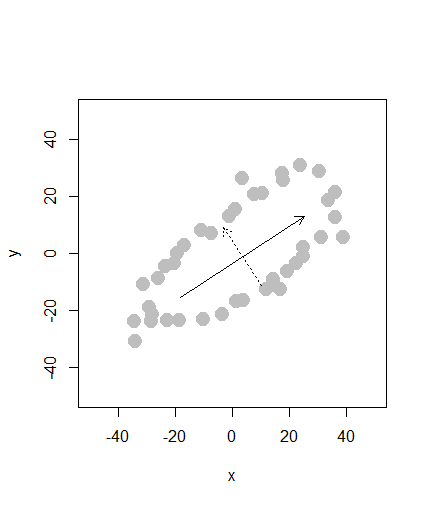
\includegraphics{images/PCA1.png}

\begin{longtable}[]{@{}ll@{}}
\caption{Standard Deviations (1, .., p=2):}\tabularnewline
\toprule
\endhead
36.96495 & 18.43857 \\
\bottomrule
\end{longtable}

\begin{longtable}[]{@{}lll@{}}
\caption{Rotation (n x k) = (2 x 2):}\tabularnewline
\toprule
\endhead
- & \(PC1\) & \(PC2\) \\
\(x\) & 0.8330720 & -0.5474046 \\
\(y\) & 0.5474046 & 0.8330720 \\
\bottomrule
\end{longtable}

\hypertarget{b.-create-a-scatterplot-whose-principal-component-vectors-do-not-seem-to-match-the-major-directions-of-variance.-show-this-visualization.}{%
\subsubsection{b. Create a scatterplot whose principal component vectors
do NOT seem to match the major directions of variance. Show this
visualization.}\label{b.-create-a-scatterplot-whose-principal-component-vectors-do-not-seem-to-match-the-major-directions-of-variance.-show-this-visualization.}}

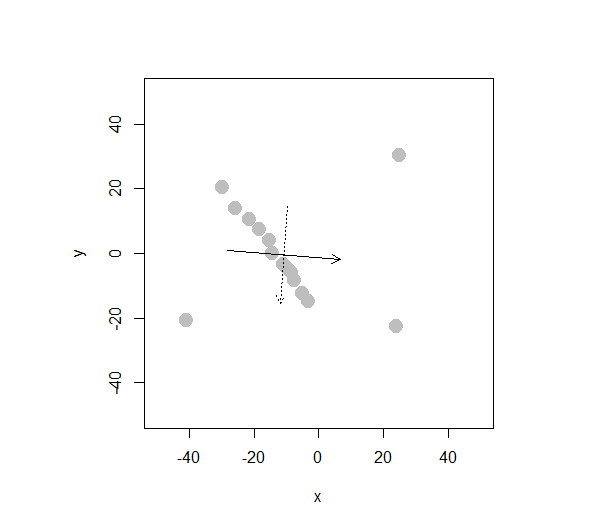
\includegraphics{images/PCA.png}

\begin{longtable}[]{@{}ll@{}}
\caption{Standard Deviations (1, .., p=2):}\tabularnewline
\toprule
\endhead
17.51977 & 14.99578 \\
\bottomrule
\end{longtable}

\begin{longtable}[]{@{}lll@{}}
\caption{Rotation (n x k) = (2 x 2):}\tabularnewline
\toprule
\endhead
- & \(PC1\) & \(PC2\) \\
\(x\) & 0.9969089 & -0.0785661 \\
\(y\) & -0.0785661 & -0.9969089 \\
\bottomrule
\end{longtable}
\end{quote}

\end{document}
